\chapter{Numerical Methods for Differential Equations}

\section{Ordinary Differential Equations (ODEs)}

\subsection{Initial Value Problems}

\todo{Only the methods used in the tutorials: Verlett, RK4, Explicit Euler}

Consider the Initial Value Problem

\begin{equation*}
	\begin{cases}
		\diff{y}{t}=
		f\left(t,y\right), & t\in\left[0,T\right]. \\
		y\left(0\right)=
		y_{0}.             &
	\end{cases}
\end{equation*}

\subsubsection{Backward Euler Method}
% https://www.youtube.com/watch?v=HeVsOss1w78
\begin{equation*}
	f\left(t_{n+1},y_{n+1}\right)
	=\diff{y}{t}\approx
	\frac{y_{n+1}-y_{n}}{\Delta t}\implies
	y_{n+1}=
	y_{n}+
	f\left(t_{n+1},y_{n+1}\right)
	\Delta t.
\end{equation*}

The local truncation error is
\begin{math}
	\mathcal{O}
	\left(\Delta t^{2}\right)
\end{math}.
The Butcher table is
\begin{math}
	\renewcommand\arraystretch{1.2}
	\begin{array}
		{c|c}
		1 & 1 \\
		\hline
		  & 1
	\end{array}
\end{math}.

\begin{equation*}
	\begin{cases}
		\diff{y}{t}=
		y\sin t^{2},       & t\in\left[0,5\right]. \\
		y\left(0\right)=2. &
	\end{cases}
\end{equation*}

\begin{equation*}
	S\left(x\right)\coloneqq
	\int_{0}^{x}\sin\left(t^{2}\right)\dl t=
	\sum_{n=0}^{\infty}
	\frac{{\left(-1\right)}^{n}x^{4n+3}}{\left(2n+1\right)!\left(4n+3\right)}.
\end{equation*}

We integrate and obtain the general solution.
\begin{align*}
	\iint
	\diff[2]{u}{x}
	\dl x
	\dl x           & =
	\iint
	e^{x}
	\dl x
	\dl x.              \\
	\int
	\diff{u}{x}
	\dl x           & =
	\int
	\left(e^{x}+C_{1}\right)
	\dl x.              \\
	u\left(x\right) & =
	e^{x}+C_{1}x+C_{2}.
\end{align*}
Now, let's apply the Robin boundary conditions.
\begin{equation}\label{eq:linearsystem}
	\left\{
	\begin{aligned}
		0
		 & =
		u\left(0\right)-
		\diff{u}{x}[x=0]=
		e^{0}+C_{1}\left(0\right)+C_{2}-
		\left(e^{0}+C_{1}\right)=
		C_{2}-C_{1}. \\
		2e
		 & =
		u\left(1\right)+
		\diff{u}{x}[x=1]=
		e^{1}+C_{1}\left(1\right)+C_{2}+
		\left(e^{1}+C_{1}\right)=
		2e+2C_{1}+C_{2}.
	\end{aligned}
	\right.
\end{equation}
El sistema~\eqref{eq:linearsystem} tiene como solución
$C_{1}=C_{2}=0$.
$\therefore$ la solución
de~\eqref{eq:poisson1drobindconditions} es
$u\left(x\right)=e^{x}$.

\begin{listing}[ht!]
	\tiny
	\centering
	\pathinputminted[frame=single,framesep=10pt,linenos,firstline=1,lastline=13,highlightlines={12}]{octave}{backward_euler.m}
	\caption{Program~\texttt{backward\_euler.m}}
	\label{code:backward_euler.m}
\end{listing}

\begin{figure}[ht!]
	\centering
	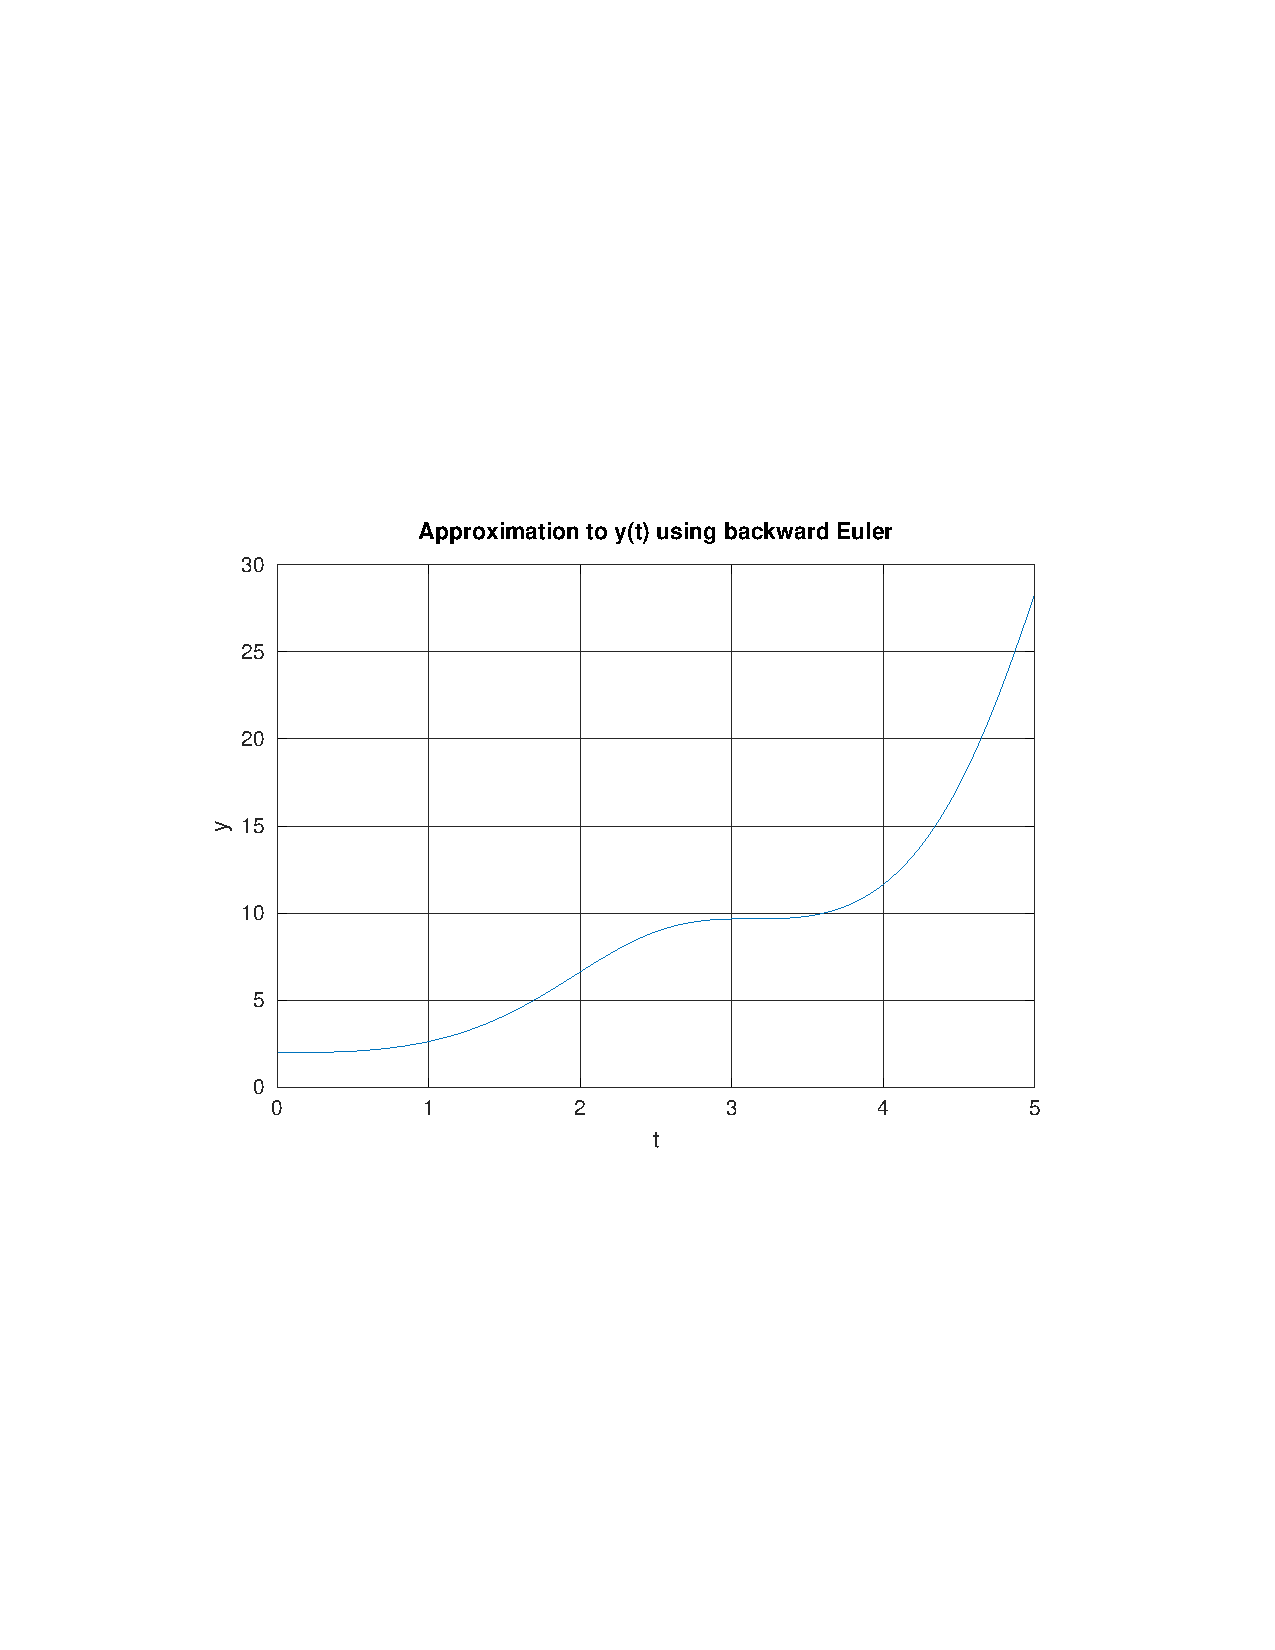
\includegraphics[width=0.55\paperwidth]{backward_euler.pdf}
	\caption{Numerical solution by the Backward Euler Method.}
\end{figure}

\begin{itemize}
	\item

	      \url{https://docs.octave.org/v9.4.0/Ranges.html}

	\item

	      \url{https://docs.octave.org/v9.4.0/Solvers.html#XREFfzero}

	\item

	      \url{https://docs.octave.org/v9.4.0/Object-Sizes.html#XREFsize}

	\item

	      \url{https://docs.octave.org/v9.4.0/Object-Sizes.html#XREFlength}

	\item

	      \url{https://docs.octave.org/v9.4.0/Trigonometry.html#XREFsin}

	\item

	      \url{https://docs.octave.org/v9.4.0/Special-Utility-Matrices.html#XREFzeros}
\end{itemize}

% \url{https://docs.octave.org/v9.4.0/Basic-Vectorization.html}
% \url{https://docs.octave.org/v9.4.0/Ordinary-Differential-Equations.html}

\subsubsection{Explicit Runge-Kutta 2}
% https://www.youtube.com/watch?v=HeVsOss1w78
\begin{align*}
	\widetilde{y}_{n+1} & =
	y_{n}+
	f\left(t_{n},y_{n}\right)\Delta t. \\
	y_{n+1}             & =
	y_{n}+
	\frac{\Delta t}{2}
	\left(
	f\left(t_{n},y_{n}\right)+
	f\left(\widetilde{y}_{n+1},t_{n+1}\right)
	\right).
\end{align*}

The local truncation error is
\begin{math}
	\mathcal{O}
	\left(\Delta t^{2}\right)
\end{math}.
The Butcher table is
\begin{math}
	\renewcommand\arraystretch{1.2}
	\begin{array}
		{c|cc}
		0 &             &             \\
		1 & 1           &             \\
		\hline
		  & \frac{1}{2} & \frac{1}{2}
	\end{array}
\end{math}.

\begin{listing}[ht!]
	\tiny
	\centering
	\pathinputminted[frame=single,framesep=10pt,linenos,firstline=1,lastline=14,highlightlines={11-13}]{octave}{RK2.m}
	\caption{Program~\texttt{RK2.m}}
	\label{code:RK2.m}
\end{listing}

\begin{listing}[ht!]
	\tiny
	\centering
	\pathinputminted[frame=single,framesep=10pt,linenos,firstline=1,lastline=81,highlightlines={41-47}]{cpp}{RK2.cpp}
	\caption{Program~\texttt{RK2.cpp}}
	\label{code:RK2.cpp}
\end{listing}

\begin{figure}[ht!]
	\centering
	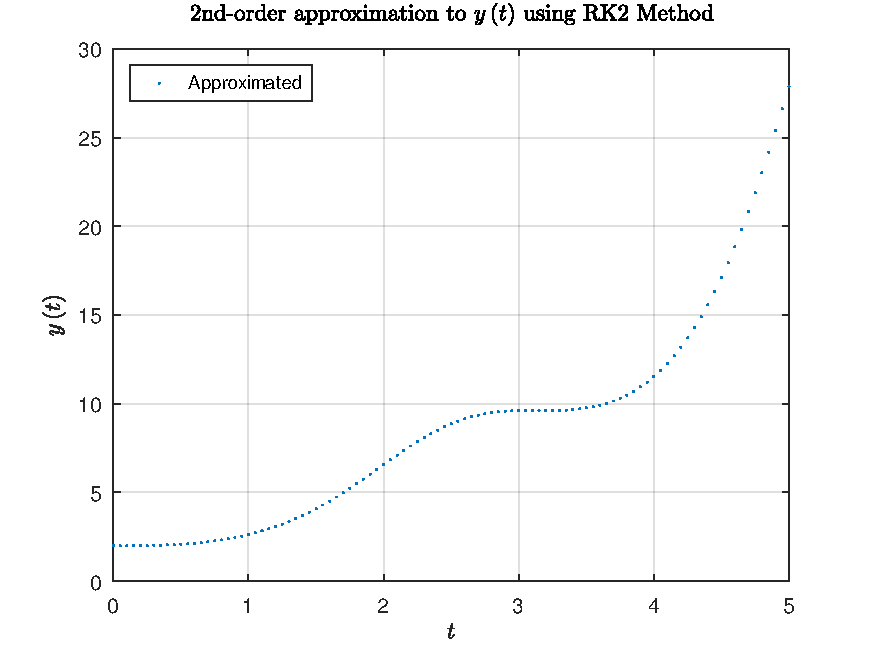
\includegraphics[width=0.55\paperwidth]{RK2.pdf}
	\caption{Numerical solution by the Runge-Kutta 2 Method.}
\end{figure}

\subsubsection{Explicit Runge-Kutta 4}
% https://jonshiach.github.io/ODEs-book/_pages/2.3_RK4_Derivation.html
% https://www.youtube.com/watch?v=qUe_kR7QoBU

\begin{align*}
	k_{1}   & =
	f\left(t_{n},y_{n}\right).                                            \\
	k_{2}   & =
	f\left(t_{n}+\frac{\Delta t}{2},y_{n}+\Delta t\frac{k_{1}}{2}\right). \\
	k_{3}   & =
	f\left(t_{n}+\frac{\Delta t}{2},y_{n}+\frac{\Delta k_{2}}{2}\right).  \\
	k_{4}   & =
	f\left(t_{n}+\Delta t,y_{n}+\Delta t k_{3}\right).                    \\
	y_{n+1} & =
	y_{n}+
	\frac{1}{6}\left(k_{1}+2k_{2}+2k_{3}+k_{4}\right).
\end{align*}

The local truncation error is
\begin{math}
	\mathcal{O}
	\left(\Delta t^{4}\right)
\end{math}.
The Butcher table is
\begin{math}
	\renewcommand\arraystretch{1.2}
	\begin{array}
		{c|cccc}
		0           &             &             &             &             \\
		\frac{1}{2} & \frac{1}{2} &             &             &             \\
		\frac{1}{2} & 0           & \frac{1}{2} &             &             \\
		1           & 0           & 0           & 1           &             \\
		\hline
		            & \frac{1}{6} & \frac{4}{6} & \frac{4}{6} & \frac{1}{6}
	\end{array}
\end{math}.

\begin{listing}[ht!]
	\tiny
	\centering
	\pathinputminted[frame=single,framesep=10pt,linenos,firstline=1,lastline=16,highlightlines={11-15}]{octave}{RK4.m}
	\caption{Program~\texttt{RK4.m}}
	\label{code:RK2.m}
\end{listing}

\begin{figure}[ht!]
	\centering
	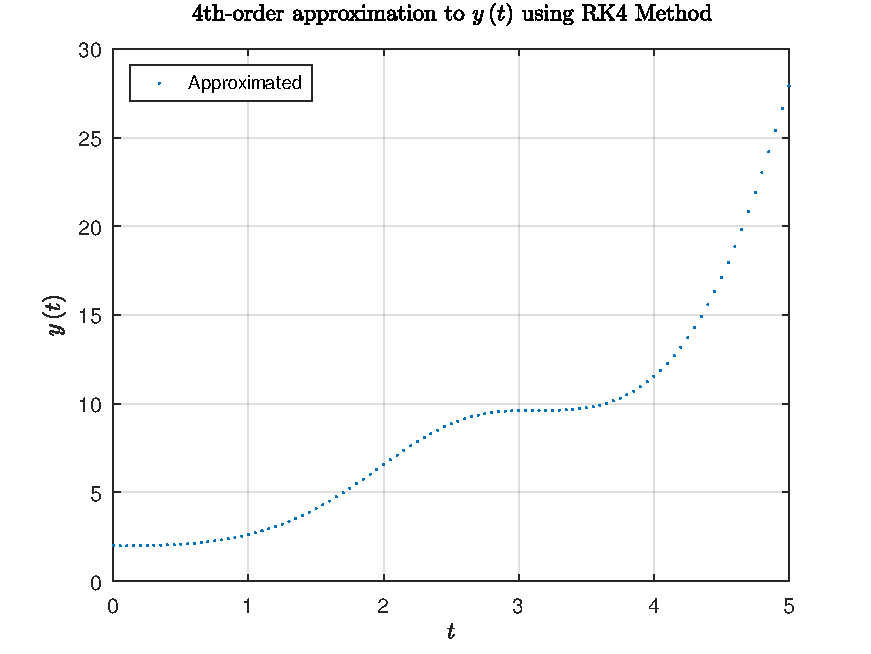
\includegraphics[width=0.55\paperwidth]{RK4.pdf}
	\caption{Numerical solution by the Runge-Kutta 4 Method.}
\end{figure}

\subsubsection{Verlett}

\subsection{Boundary Value Problems}

\section{Partial Differential Equations (PDEs)}

\subsection{von Neumann Stability Analysis}

\subsection{Convergence and Error Estimation}
